\documentclass[english]{article}
\usepackage[T1]{fontenc}
\usepackage[latin9]{inputenc}
\usepackage{geometry}
\geometry{verbose,tmargin=3cm,bmargin=3cm,lmargin=3cm,rmargin=3cm}

\makeatletter
\usepackage{url}

\makeatother

\usepackage{babel}
\usepackage{xcolor}
\usepackage[backend=bibtex, style=ieee]{biblatex}
\addbibresource{bibliography.bib}
\usepackage[hidelinks]{hyperref}
\usepackage{graphicx}
\graphicspath{ {./images/} }

\title{Research Plan for Multi-Agent Path Finding with Matching using A* with OD and ID}
\author{Ivar de Bruin}
\date{\today}

\newcommand{\namelistlabel}[1]{\mbox{#1}\hfil}
\newenvironment{namelist}[1]{%1
\begin{list}{}
    {
        \let\makelabel\namelistlabel
        \settowidth{\labelwidth}{#1}
        \setlength{\leftmargin}{1.1\labelwidth}
    }
  }{%1
\end{list}}

\begin{document}
\maketitle

\begin{namelist}{xxxxxxxxxxxxxxxxxxxxxxxxxxxxxxxxxxxxxxx}
\item[{\bf Title:}]
	Multi-Agent Path Finding with Matching using A* with OD and ID
\item[{\bf Author:}]
	Ivar de Bruin
\item[{\bf Responsible Professor:}]
	Mathijs de Weerdt
\item[{\bf Other Supervisor:}]
	Jesse Mulderij
%\item[{\bf (Required for final version) Examiner:}]
%	Another Professor (\emph{interested, but not involved})
\item[{\bf Peer group members:}]
	Robbin Baauw, Jonathan D\"onszelmann, Jaap de Jong, Thom van der Woude
\end{namelist}

\tableofcontents

\section{Background of the research}
The Dutch Railways (NS) is tasked with maintaining trains during the night. 
The trains are routed to shunting yards where they can be cleaned and receive maintenance. 
Here there is an NP-hard problem called the Train Unit Shunting and Servicing (TUSS) problem. 
One of the main questions in this problems is with regards to the capacity of these shunting yards. 
To try and establish an upper bound to this capacity we try to find a relaxation to the problem. 

The NP-hard Multi-Agent Path Finding (MAPF) describes multiple agents on a graph, moving from a start node to a goal node while avoiding collisions. 
In this problem we try to minimize the sum of individual costs (SIC).
To make this problem into a relaxation of the TUSS problem we also need to introduce matching, as there is no exact assignment per train for a destination but rather per class or type of train.
\\\\%TODO: describe current state
{\color{red}Description of current state of the research field to be added later}


\section{Research Question}
The main question that will be answered in this paper is: How can the MAPF algorithm A* with ID and OD be used to solve a relaxation of the TUSS problem when it is expanded with matching. We can then look at the following sub-questions:
\begin{itemize}
	\item Which matching algorithm performs best when combined with A* with OD and ID
	\item How does this combined algorithm perform compared to other MAPF algorithms expanded with matching?
	\item Under which conditions should this algorithm be used?
	\item Under which conditions should this algorithm not be used?
\end{itemize}
%TODO: Fix and expand
{\color{red}Will be expanded and improved later this week}

\section{Method}
To complete this research the following things need to be accomplished:
\begin{itemize}
	\item Implement A* with ID and OD to be extended with matching
	\item Extend this basic version with a matching method to solve MAPF-M
	\item Use created benchmarks to analyse the performance of the algorithm compared to other versions and other algorithms
	\item Use this analysis to improve performance and enhancements of the algorithm
\end{itemize}

These benchmarks will be run on a website maintained by one of my peers (Jonathan D\"onszelmann). This will mean all algorithms are tested under the same conditions allowing for a fair comparison. All algorithms will also be developed in Python to further aid the fairness of this comparison.

\section{Planning of the research project}
Here I will explain what I plan to spent each week on, I will also include a table of the deadlines and other things from the university as a clear overview of deadlines.

\subsection*{Week 1: Orientation}
The first week will be spent on orientation. What is the current state of the field?  How does A* ID OD really work. How can I make it? etc.
\\\\
During this week I will also orientate myself on the different deadlines and lectures we have. For example how to prepare for each one.
\\\\
For this orientation I will also be reading quite a few papers starting with Standley's paper on A* with ID and OD \cite{AStarIDOD_standley_2010}, Stern et al. paper on Multi-Agent pathfinding\cite{stern2019multiagent} and Mulderij et al. paper on the TUSS problem\cite{mulderij2020train}. As well as any papers that follow from that that seem relevant.
\\\\
This orientation should then finally allow me to make the final version of this research plan at the end of the week.

\subsection*{Week 2: Developing a basic version of A*+ID+OD}
This week will be spent on creating a basic MAPF solver in A*+ID+OD. This will make me more familiar with the algorithm as well as give me something to extend. This week there is also the research plan presentation that needs to be prepared.

\subsection*{Week 3: Research matching}
This week I will finish the algorithm if I did not finish it last week. 
After creating a MAPF solver I will need to research how to introduce matching to it. 
For this I will look at some papers but as matching with MAPF is not a research area with a lot of publications quite a bit of this research will be done through experimentation.
Once I have an idea of what to do I will start extending the basic algorithm with matching.

\subsection*{Week 4: Matching and preparing midterm}
This week I will continue with the addition of matching to the algorithm. I will also start preparing for the midterm presentation on Wednesday of week 5

\subsection*{Week 5: Midterm presentation}
This week is the midterm presentation. Besides this I will start on the paper as well as perhaps start comparing the benchmarks with my peers.

\subsection*{Week 6: Improve performance}
This week will be about improving performance and running further comparisions with my peers. I will also continue using the lectures from university to continue working on the first draft of my paper.

\subsection*{Week 7: Start final rounds of improvement and finish draft v1}
This week I will figure out what can still be improved in the algorithm as well as finish the draft of my paper.

\subsection*{Week 8: Draft reviews}
This week I will need to review others papers as well as improve my own. I will also be running most of the final experiments so version 2 of the paper draft can contain this data.

\subsection*{Week 9: Draft version 2}
This week draft version 2 needs to be finished. This week I will also finish the work on the code and the experiments.

\subsection*{Week 10: Work on final paper and poster}
This week the paper should be finished and the poster mostly finished.

\subsection*{Week 11: Presentation}
This week the poster will be handed in and the final presentation be prepared and given.

\pagebreak
\subsection*{Planning overview}
\begin{figure}[h]
	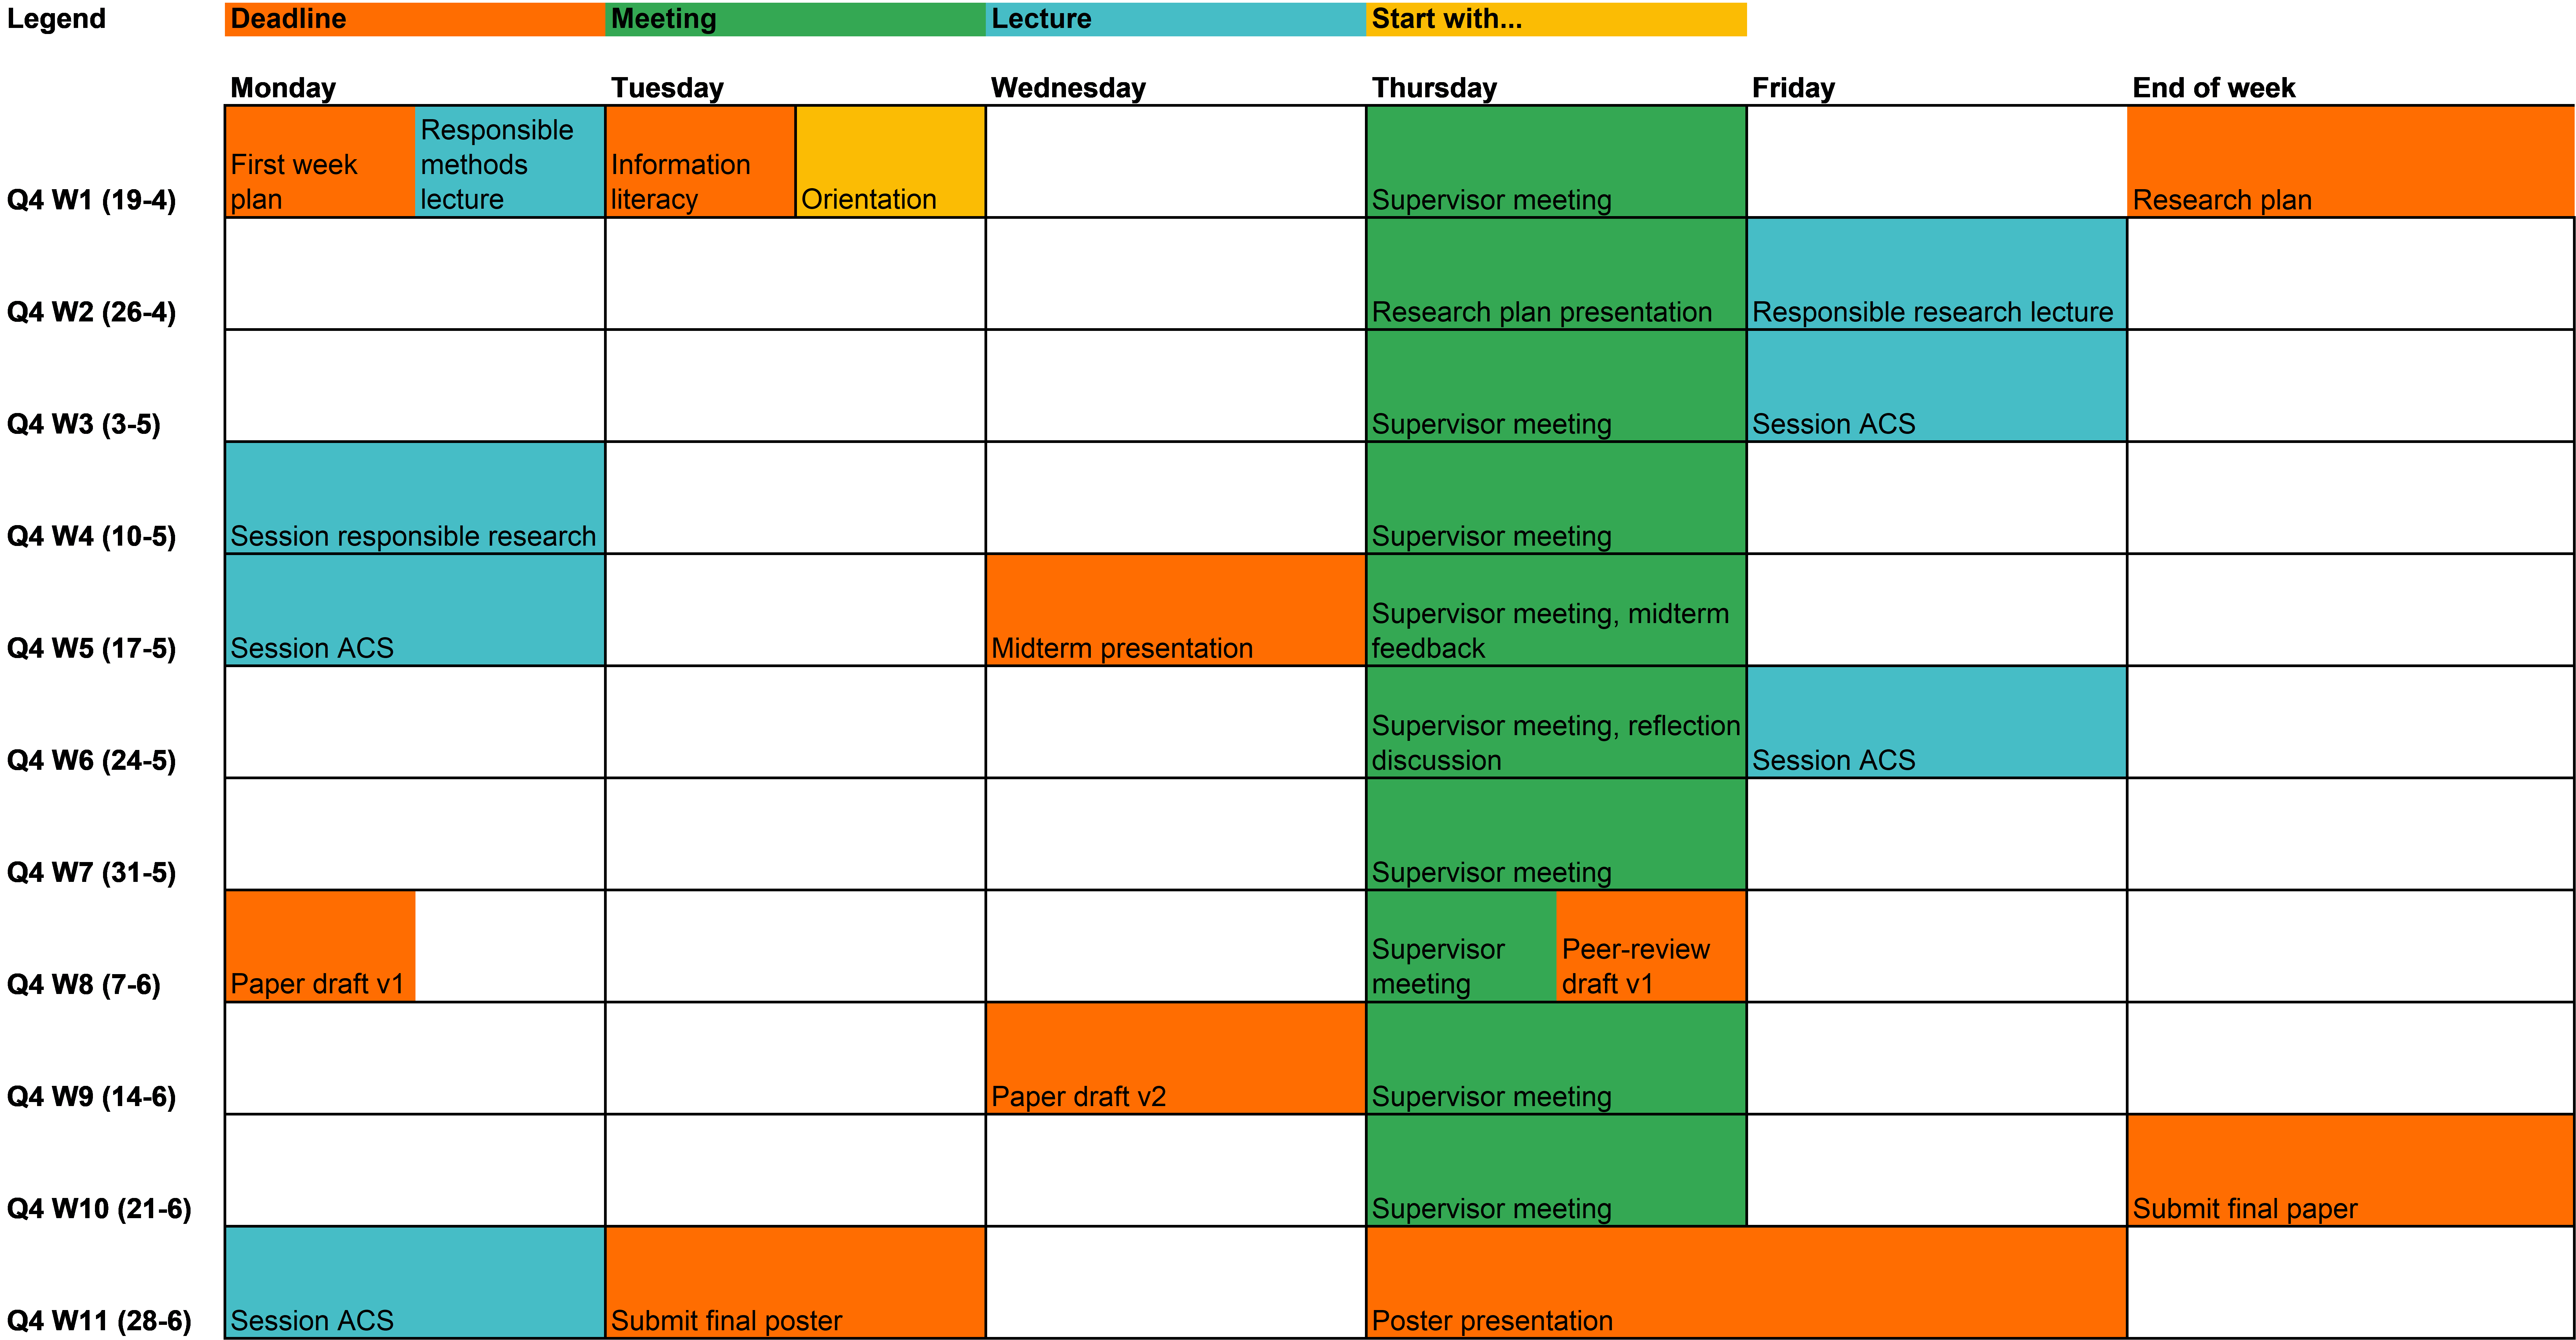
\includegraphics[width=\linewidth]{Planning}
	\centering
	\caption{Draft planning overview}
\end{figure}


\printbibliography

%for convenience we use here the in-document bibliography
%\begin{thebibliography}{9}
%\bibitem{wessen} Ken Wessen, Preparing a thesis using \LaTeX~, private
%communication, 1994.
%\end{thebibliography}

\end{document}
